\section{Discussion and experimental results}\label{disc}
%What 'advice' to give to the reader? Discuss difficulties (e.g. tosca) and such.

% include preliminary performance measurements, emphasize that it's outside the scope of our research, no real conclusions should be made, just observations, this needs to be made very clear

%Metadata, rules, web resolver link or not etc. all depending on \gls{pid} and cloud provider.


%%% ZHAO feedback
    %   - how do they work as a whole
    %   - Demonstrate its usage via example: show all components
    %   - some performance study etc?
    %   - summarize what you did
    %   - novelty (quality of being new and original)
    %   - weakness

% what is the value of this research?
% distribution of data
% deployment of ndn network by using cloud
% request pids but actually query the ndn network

% weaknesses
% only 3 pid types in poc
% not implemented full tosca deployment
% more detailed planning if more data is fed to planning method

In this section we will discuss our proposed solutions that we explored in order to answer the research questions. Furthermore, we will discuss some preliminary \gls{ndn} performance of our proof of concept in section \ref{discussion-performance}.

% RESEARCH QUESTION NDN
% How to plan and manage an NDN's life cycle with scalability in mind?

% To answer this research question we need to analyze the known scalability problems in \gls{ndn}. Furthermore, the term scalability needs to apply to manageability as well. If scaling in or out in terms of resources is made uncomplicated, the efforts needed to manage this infrastructure needs to stay the same.

%     \item[--] Which \gls{ndn} scaling problems are known?
%     \item[--] Which method can be used to plan an NDN?
%     \item[--] How to deploy an \gls{ndn} with scalability in mind?



% FOLLOWING NEEDS TO BE ADDED ACCORDING TO FINAL FEEDBACK

%       first come back to the research questions and analyse how and why the questions have been solved - highlight the value that has been conveyed to the reader

%       address the needs (business) for research clouds and connect the research question to it clearly and how it's answered

%       refer back to related work (field of big science) where \gls{ndn} proved to be a success in order to improve data distribution and network efficiency

% highlight that with more users (which is expected with the growth of research clouds and their users) - the caching will come more to use

%   address that this is a general approach to the problems faced by research clouds

%   discuss that udt could potentially improve UDP-like traffic

%       "McCabe is a published method used by e.g. NASA network engineers to maintain their infrastructure" - Something along these lines, can also be in related work (the NASA part) -   But it should be clear that this is a published method to guide large deployments methodologically.

%       address that for accurate planning it is needless to say that monitoring of infrastructure is required

%       \gls{ndn} facilitates data distribution scalability, the deployment method is used to facilitate a manageable deployment. I will try to make this distinction in more detail in the discussion section.

Research clouds make large datasets available to many users, with growth expected in the future. Lim et al. researched and proved the effectiveness of \gls{ndn} for big science workflows, as discussed in section \ref{introduction-related-work}. However, the data distribution benefits provided by \gls{ndn} would become unscalable without the means to maintain the life cycle. Therefore, our research developed and tested a method for planning and managing the \gls{ndn} life cycle on a larger scale by utilizing cloud providers.

The method is a general solution for planning and deploying the \gls{ndn} regardless of the research cloud its size. As demonstrated in section \ref{planning-deploying}, we have allowed the ability to flexibly scale a data distribution network. Which, with the use of the \gls{tosca} standard, could be deployed in different \gls{tosca}-ready cloud providers without alteration. This flexibility allows the data distribution network to scale easily and make management uncomplicated. However, TOSCA-ready cloud providers are still rare, for our method to be more relevant, a wider adoption is needed.

The McCabe method \cite{mccabe2010network} is utilized to establish the requirements and high-level design of the \gls{ndn} in TOSCA. McCabe offers a proven, yet simple methodological approach for defining the design goals, which are then used to define the \gls{tosca} descriptions.

Furthermore, in research clouds identification services are used and utilize different \gls{pid} schemas. Our research created a better integration between the identification services and the data transmission services. Where traditionally IP is used for host-to-host communication, our solution utilizes \gls{ndn}.


%       The work you did with NDN/PID is to investigate how identification services and transmission services can be better integrated. The current world: \gls{pid} is publication, and transmission is based on other network protocols. Our motivtion is to investigate if PID, caching, digital object discovery, routine etc. can be all implemented using the \gls{ndn} technology.



%       address that wide adoption of tosca is needed for this method, at present time this is not the case, but the research and adoption look promising

%       address that research clouds have a federated nature, while this train of thought assumes a centrally controlled method of deployment - approach this like i) as internal data-sharing platform per infrastructure, ii) as a third party data-sharing platform, one can deploy and operate for multiple infrastructure. The business model is not the key focus of the paper; but it provides technical possibility to make those servies.

% only address this part below as 'based on related work' to clearly define what the contribution was
NDN requires a different namespace format than \glspl{pid}, this is due to the incompatible nature of these namespaces. Thus a translation was needed from the \gls{pid} to the \gls{ndn} namespace, this solution was demonstrated in section \ref{pid-poc} and integrated in our proof of concept as discussed in section \ref{planning-ndn}.

% needs to come back first to the research questions, then provide how this was answered
Furthermore, the focus was on developing an extendable solution for new \gls{pid} schemas. Our solution succeeded by making use of regular expressions to match with a certain \gls{pid} type, and then call the associated function in order to do the translation to an \gls{ndn} name. Furthermore, this solution was integrated into our \gls{ndn} proof of concept. We were unable to implement our solution into the existing \gls{naas4pid} software, as this was not made publicly available.

% relate this transparcy part to a specific research question
To cache an object in our \gls{ndn} proof of concept, the user is required to first request the object from the \gls{pid} server. The object can then be requested in \gls{ndn} afterwards. Therefore, providing transparency for the user by not requiring any further user input, has not been implemented but can be achieved as described in section \ref{results-pid}. In a previous study, user input was required after translation, which is also the case in our current proof of concept. In section \ref{pid-poc} we describe how transparency for a user can be achieved. This is accomplished due to the gateway’s responsibility for \gls{pid} to \gls{ndn} translation and the object retrieval which is taken care of by the client. Our solutions are made freely available under the \gls{gpl}\footnote{\url{https://github.com/AquaL1te/rp2}}.

An alternative, less complicated design is also possible, where the client does not have to support \gls{ndn}. This is accomplished by making the gateway communicate over the \gls{ndn} protocol to an \gls{ndn} and IP to the client. A client that wants to retrieve a object, uses this gateway as their resolver. The gateway retrieves the object from \gls{ndn} (or from the \gls{pid} server if it is not already in NDN) and sends this back to the client through IP. However, the gateway needs to cache the object before sending it to the client, which can cause delay for the client when retrieving an object. This design does not require the client to support \gls{ndn} as it can retrieve objects through the gateway with regular web browsers, which communicate with the gateway over HTTP. 
% (For each \gls{pid} type one gateway? So you only have to add another gateway when a new \gls{pid} type is introduced?)

% You can explain that the \gls{ndn} provides different opportunities for data infrastructures: i) as internal data-sharing platform per infrastructure, ii) as a third party data-sharing platform, one can deploy and operate for multiple infrastructure. The business model is not the key focus of the paper; but it provides technical possibility to make those servies.

% Focus on the needs and business scenarios where we need scaling, and analyze how you did can enable those scaling. Other parts will have to be left as future work.















%This is due to gateway’s responsibility for \gls{pid} to \gls{ndn} translation and the object retrieval, which is taken care of by the client.
%combining the scripts that we have created by adding a conditional statement. This statements checks whether an object is already published in \gls{ndn}.

% The second problem statement has been addressed in section \ref{planning-ndn}, where \gls{ndn} was identified as a potential solution for the data distribution and network load problem. Therefore, a method of planning and deploying such a network was explored in detail and tested. It was concluded that a scalable and manageable data distribution network can be realized by using a \gls{nfv}-style of an \gls{ndn} deployment. Of which the life cycle can be managed by the use of \gls{tosca} templates. However, a full \gls{tosca} orchestrated deployment could not be demonstrated. This was due to the fact that \gls{tosca} orchestrators are still in development. However, Kubernetes was used as a substitution to demonstrate the deployment level on a higher level in the deployment chain. In practice, Kubernetes would be deployed by a \gls{tosca} orchestrator as well. Compared to traditional network management, NVF provides more flexibility, by the use of a centrally control the virtual \gls{ndn} functions in the network. If the behavior of the users change and thus the stress on the network, our solution will be able to adjust the network without adding extra complexities.





%Discussion or future work.
% For our proof of concept we created two scripts for the client side and two scripts for the gateway to demonstrate our design. The gateway and client are conceptually part of the \gls{ndn} network we have setup with Kubernetes and can be scaled in or out. The responsibility of the scripts on the client side is to retrieve a requested object either from the \gls{pid} server or from \gls{ndn}. The scripts that are implemented in the gateway send either the \gls{pid} link or the name in \gls{ndn} to the client for retrieval of the requested object after translation. This depends on the object being published in \gls{ndn} or not.

%Usually, \gls{ndn} operates with in-network caching. However, we used \texttt{ndnputchunks} to cache objects in \gls{ndn} in our proof of concept, which does not serve a file but works with a standard input stream. Data is cached in-memory and takes up to three times the size of the object for encoding \cite{ndnput-mem}. For using a persistent file cache we already compiled the base image of our proof of concept with repo-ng\footnote{https://github.com/named-data/repo-ng} as that utilizes
%is part 
%the \gls{cxx} application we already use. Repo-ng is an open source project and is used to set up a data repository for a persistent file cache.

% For supporting multiple \gls{pid} types, we demonstrated the use of three \gls{pid} types in our proof of concept. This already proves that supporting multiple \gls{pid} types is possible. Adding more \gls{pid} types to our proof of concept, such as the ones described in Karakannas' research \cite{icn-bd} is possible but we see this more as work for an implementation.

%TCP \gls{pid} part still has to be adjusted to new \gls{pid} server. 
%> Done
%"NDN is not designed for retrieving data objects with big sizes", as Zhao stated. 
%It is meant for "large datasets" (which could be a lot of small files) and not "large objects". 
%Maybe that's why we don't see that much of a difference between \gls{ndn} vs TCP/IP for a 1000MB object in comparison to \gls{ndn} vs TCP/IP for a 100MB object... 
%Should we also state this and remove the 1000MB benchmark and run some benchmarks with a 10MB file? 
%> Done
%First time is not taken into account. So results are based on direct link between consumer and router where the data is cached.

\subsection{Preliminary performance measurements}
\label{discussion-performance}
In this section we will briefly discuss the preliminary performance of our \gls{ndn} with \gls{pid} interoperability proof of concept. The results gathered were merely based on best-effort test scenarios and are inconclusive. Therefore, further and more detailed research is required, which we will discuss in more detail in future work (section \ref{fut}). 


We used for both TCP/IP and \gls{ndn} the default values.
For TCP/IP, we did not tweak the MTU values and kept the TCP parameters to their defaults, such as the default Linux TCP congestion algorithm; Cubic. For the TCP/IP benchmarks we used the the \texttt{urllib.request} Python module, which uses the HTTP 1.1 protocol over TCP \cite{urllib}. For \gls{ndn}, we used the default MTU setting when creating a face (8800) with \texttt{nfdc} (part of the \gls{cxx} application) and did not tweak any of the parameters, which are highlighted in section \ref{fut}. For publishing objects in \gls{ndn}, we used the default settings of \texttt{ndnputchunks}, which has a MTU of 4400. The underlying technology is still IP in \gls{ndn}. However, \gls{ndn} uses hop-by-hop fragmentation. This technology enables fragmentation at each hop if needed. Which means that the whole network no longer needs to limit its MTU size to the smallest denominator \cite{ndn-mtu}.
% We want to highlight that the results we present in figure \ref{fig:perftest-1} and \ref{fig:perftest-2} are preliminary. A range of parameters can be used to optimize \gls{ndn} network performance.

The architecture used in our experiments is as follows. The \gls{ndn} consumer and router container reside on 'nimes', while the \gls{ndn} producer and router reside on 'mulhouse'. Furthermore, they are interconnected via the internet, using the Kubernetes overlay network as shown in section \ref{planning-architecture} figure \ref{fig:high-level-network-design}. As the connection is routed over the internet, latency can occur as it depends on the path a packet takes. The tool \texttt{traceroute} shows that there are no intermediate hops between 'nimes' and 'mulhouse'. The disk throughput of the server where the containers reside has a write speed of 180MB/s. Network latency is around 200 microseconds, measured by the tool \texttt{arping}.
The preliminary performance results of our Handle \gls{pid} server and the \gls{ndn} are illustrated in boxplots (figure \ref{fig:perftest-1}, \ref{fig:perftest-2}, \ref{fig:perftest-3}, \ref{fig:perftest-4} and \ref{fig:perftest-5}). We ran the following performance tests within our proof of concept using a 10MB, 100MB, 250MB, 500MB and a 1000MB data object. We performed the performance tests ten times for each object size and protocol and are processed in the illustrated boxplots. The different object sizes were chosen in order to determine if there is a certain trend between the object size and performance. This performance trend is illustrated in figure \ref{fig:perftest-6} and shows the average of the test runs. We can observe that \gls{ndn} over UDP outperforms the TCP/IP connection used for retrieving data objects from the Handle \gls{pid} server that we setup with all chosen object sizes. Furthermore, \gls{ndn} over TCP outperforms \gls{ndn} over UDP. This result correlates with the research done by Lim et al., as discussed in section \ref{introduction-related-work-ndn}. The line chart shown in figure \ref{fig:perftest-6} shows that the lines converge after the 250MB mark. Which means that the relative difference between \gls{ndn} and TCP/IP becomes smaller with object sizes bigger than 250MB. This is due to \glspl{ndn} nature of handling big object sizes. These can cause a performance problem, because the cost of retransmission when interests are retransmitted (or re-issued) becomes unsustainably high \cite{ndn-objects}. % Their research concludes that \gls{ndn} provided performance improvements compared to classical climate data delivery techniques based on TCP/IP. In addition to this, \gls{ndn} over TCP demonstrated a more reliable and faster performance due to the allowance of larger dynamic window sizes and congestion control.

\begin{figure}[H]
\centering
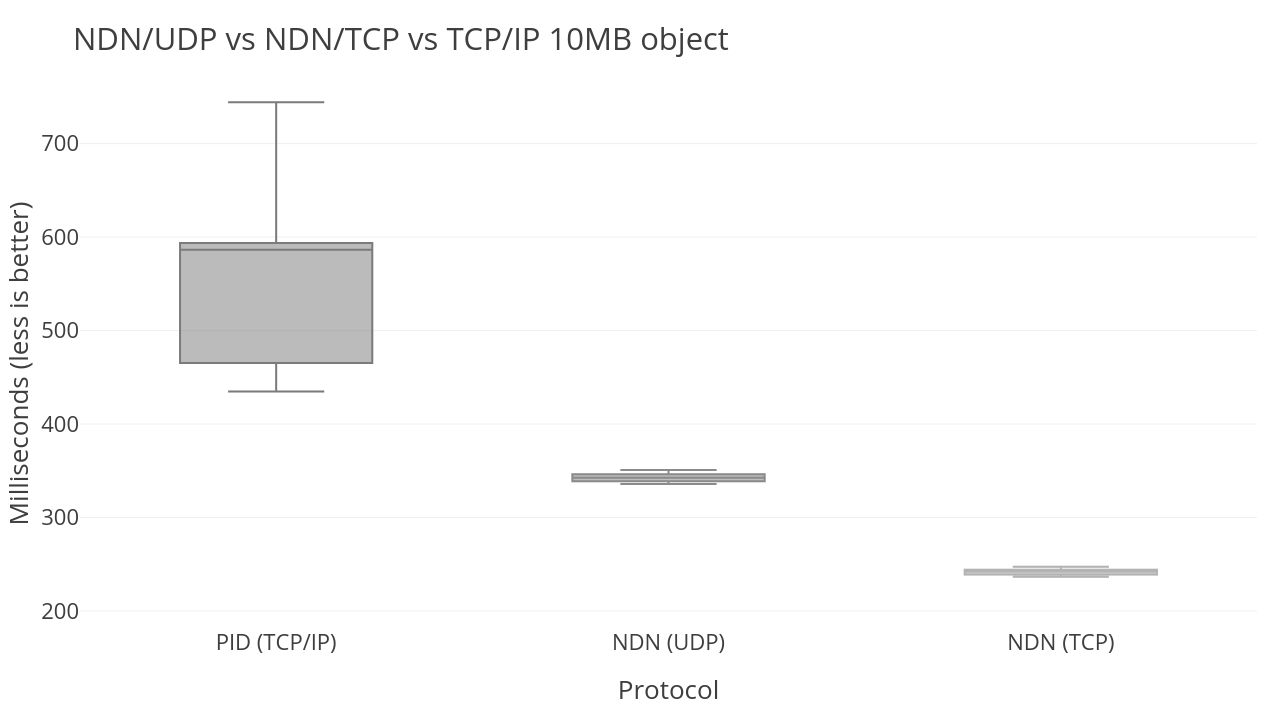
\includegraphics[scale=0.43]{Images/bench10MB_grey.png}
\caption{Performance test TCP/IP vs \gls{ndn} with a 10MB object.}
\label{fig:perftest-1}
\end{figure}

\begin{figure}[H]
\centering
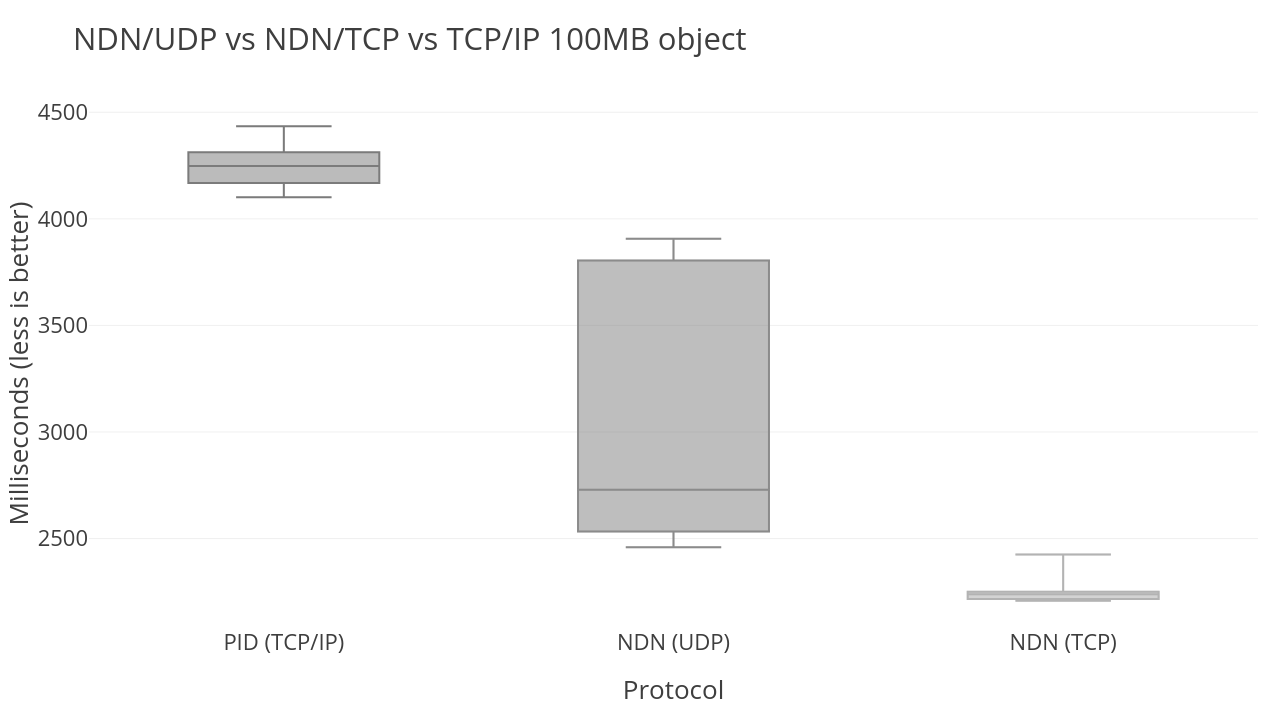
\includegraphics[scale=0.43]{Images/bench100MB_grey.png}
\caption{Performance test TCP/IP vs \gls{ndn} with a 100MB object.}
\label{fig:perftest-2}
\end{figure}

\begin{figure}[H]
\centering
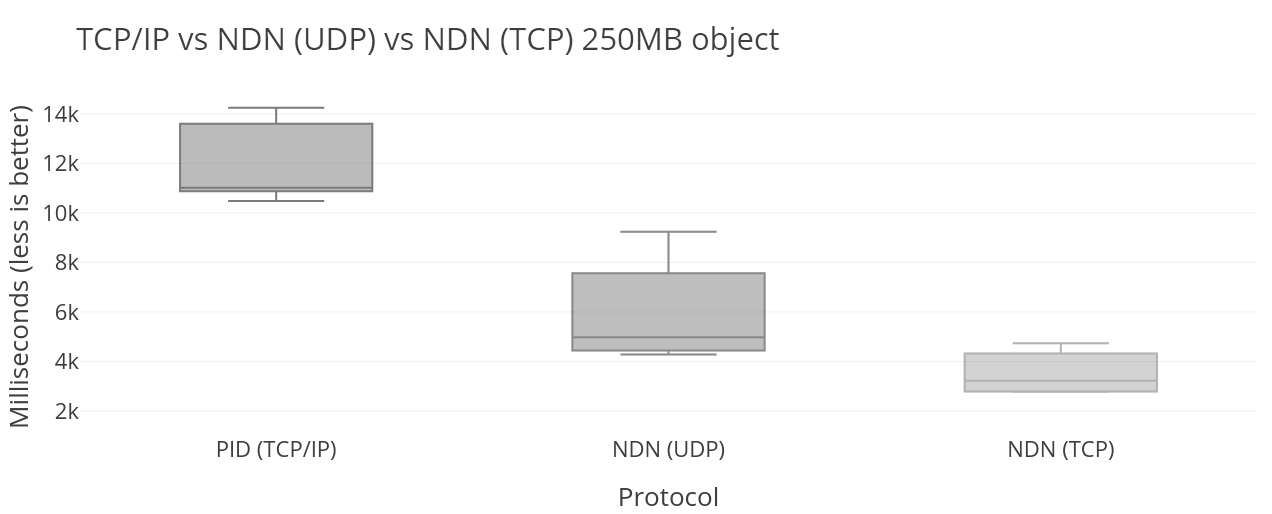
\includegraphics[scale=0.43]{Images/ndn_tcpip_250_grey.png}
\caption{Performance test TCP/IP vs \gls{ndn} with a 250MB object.}
\label{fig:perftest-3}
\end{figure}

\begin{figure}[H]
\centering
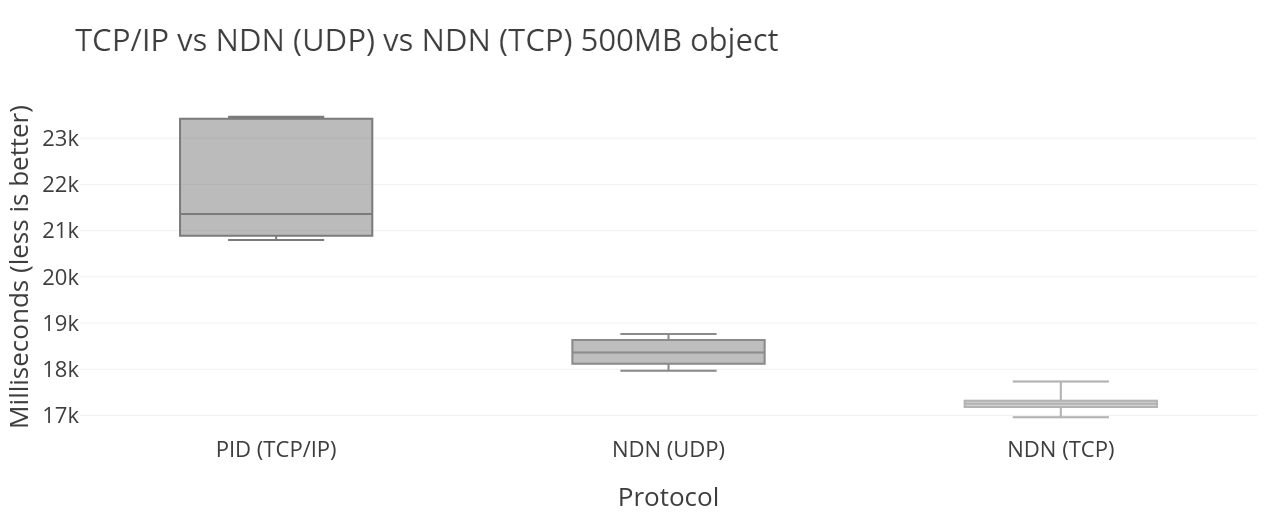
\includegraphics[scale=0.43]{Images/ndn_tcpip_500_grey.png}
\caption{Performance test TCP/IP vs \gls{ndn} with a 500MB object.}
\label{fig:perftest-4}
\end{figure}

\begin{figure}[H]
\centering
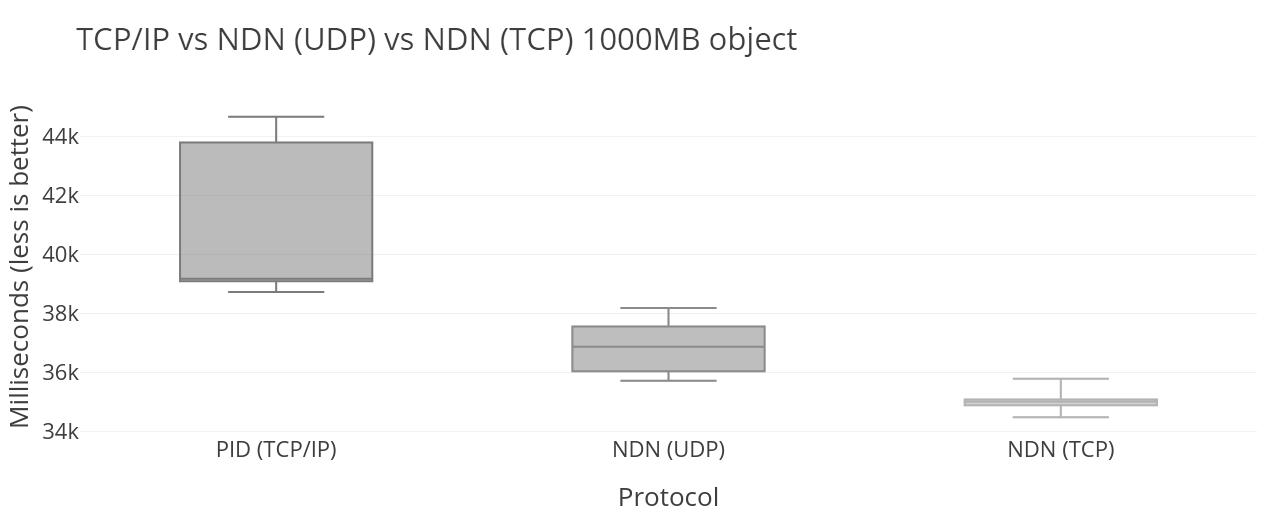
\includegraphics[scale=0.43]{Images/ndn_tcpip_1000_grey.png}
\caption{Performance test TCP/IP vs \gls{ndn} with a 1000MB object.}
\label{fig:perftest-5}
\end{figure}

\begin{figure}[H]
\centering
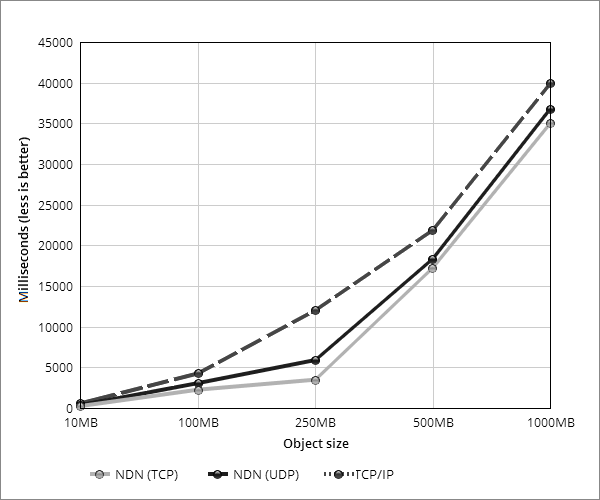
\includegraphics[scale=0.7]{Images/linechart5.png}
\caption{Object size to performance relation.}
\label{fig:perftest-6}
\end{figure}

When observing the results, we can see that it takes roughly more than four seconds to retrieve a 100MB object over TCP/IP, which does not seem to be optimal. 
%is not optimal as a 1Gbps Ethernet connection is used for the benchmarks. 
It seems that our Handle \gls{pid} server, which is set up with \texttt{cordra-1.0.7} software is the bottleneck. Since we got faster results when retrieving the Linux kernel for example. We can retrieve a 102MB Linux kernel in ${\sim}1$ second within a container in our proof of concept. This seems to be faster than the default \texttt{ndnputchunks} settings with a MTU of 4400. When raising the MTU to 8800 for publishing a object in \gls{ndn} with \texttt{ndnputchunks}, to reduce the number of signatures needed to transmit a object, we can observe that the average time to retrieve an object through \gls{ndn} takes less than a second (${\sim}850$ milliseconds). 
When retrieving a object over \gls{ndn} UDP with a MTU set to 8800 in \texttt{ndnputchunks}, we cannot observe any difference with our results shown in figure \ref{fig:perftest-2} with a MTU of 4400 over \gls{ndn} UDP. This may be caused by UDP's limitations in \gls{ndn} as described in section \ref{introduction-related-work-ndn}. 

%However, in this case we tweaked the default \texttt{ndnputchunks} settings for publishing a file in \gls{ndn}, but the default face settings are already set on 8800 when creating a face.


% TO-DO: 
% - Mention \gls{tosca} difficulties.
% - Preliminary benchmark results (PID server on nimes)
% high-availability kubernetes + persistent volumes + ndn cache